% CV802 Sub-project 3 -- one-page report (CVPR camera-ready style); references on page 2.
% Build: cd docs/report && python build_tables.py && pdflatex main && bibtex main && pdflatex main && pdflatex main
\documentclass[10pt,twocolumn,letterpaper]{article}
\usepackage{cvpr}
\usepackage{microtype}
\usepackage{booktabs}
\definecolor{cvprblue}{rgb}{0.21,0.49,0.74}
\usepackage[breaklinks,colorlinks,allcolors=cvprblue]{hyperref}
\def\paperID{}\def\confName{CV802}\def\confYear{2025}
\setlength{\abovedisplayskip}{2pt}\setlength{\belowdisplayskip}{2pt}
\renewcommand{\paragraph}[1]{\vspace{1pt}\noindent\textbf{#1}\hspace{0.4em}}
\makeatletter
\renewcommand\section{\@startsection{section}{1}{\z@}{-5pt plus -1pt}{2pt}{\large\bf}}
\patchcmd{\@maketitle}{\vskip .375in}{\vskip -0.05in}{}{}
\patchcmd{\@maketitle}{\vspace*{24pt}}{\vspace*{8pt}}{}{}
\makeatother
\captionsetup{skip=3pt}
\newcommand{\TfPSNR}{26.35}
\newcommand{\TfFPS}{1}
\newcommand{\TfMin}{42}
\newcommand{\GsPSNR}{27.53}
\newcommand{\GsFPS}{366}
\newcommand{\GsMin}{7}
\newcommand{\GsOurs}{106}
\newcommand{\GsZoomOut}{24.25}
\newcommand{\MipPSNR}{27.53}
\newcommand{\MipFPS}{594}
\newcommand{\MipMin}{10}
\newcommand{\MipOurs}{104}
\newcommand{\MipZoomOut}{28.63}
\newcommand{\FullPSNR}{19.71}
\newcommand{\FullFPS}{98}
\newcommand{\FullMin}{33}


\title{Novel Views of a Person from 125 Photos: NeRF, TensoRF, 3DGS and Mip-Splatting}
\author{Anas Khan \quad MBZUAI \quad CV802 Sub-project 3: Novel-view Synthesis}

\begin{document}
\pagestyle{empty}\thispagestyle{empty}
\twocolumn[{\renewcommand\twocolumn[1][]{#1}%
\maketitle\vspace{-34pt}
\begin{center}
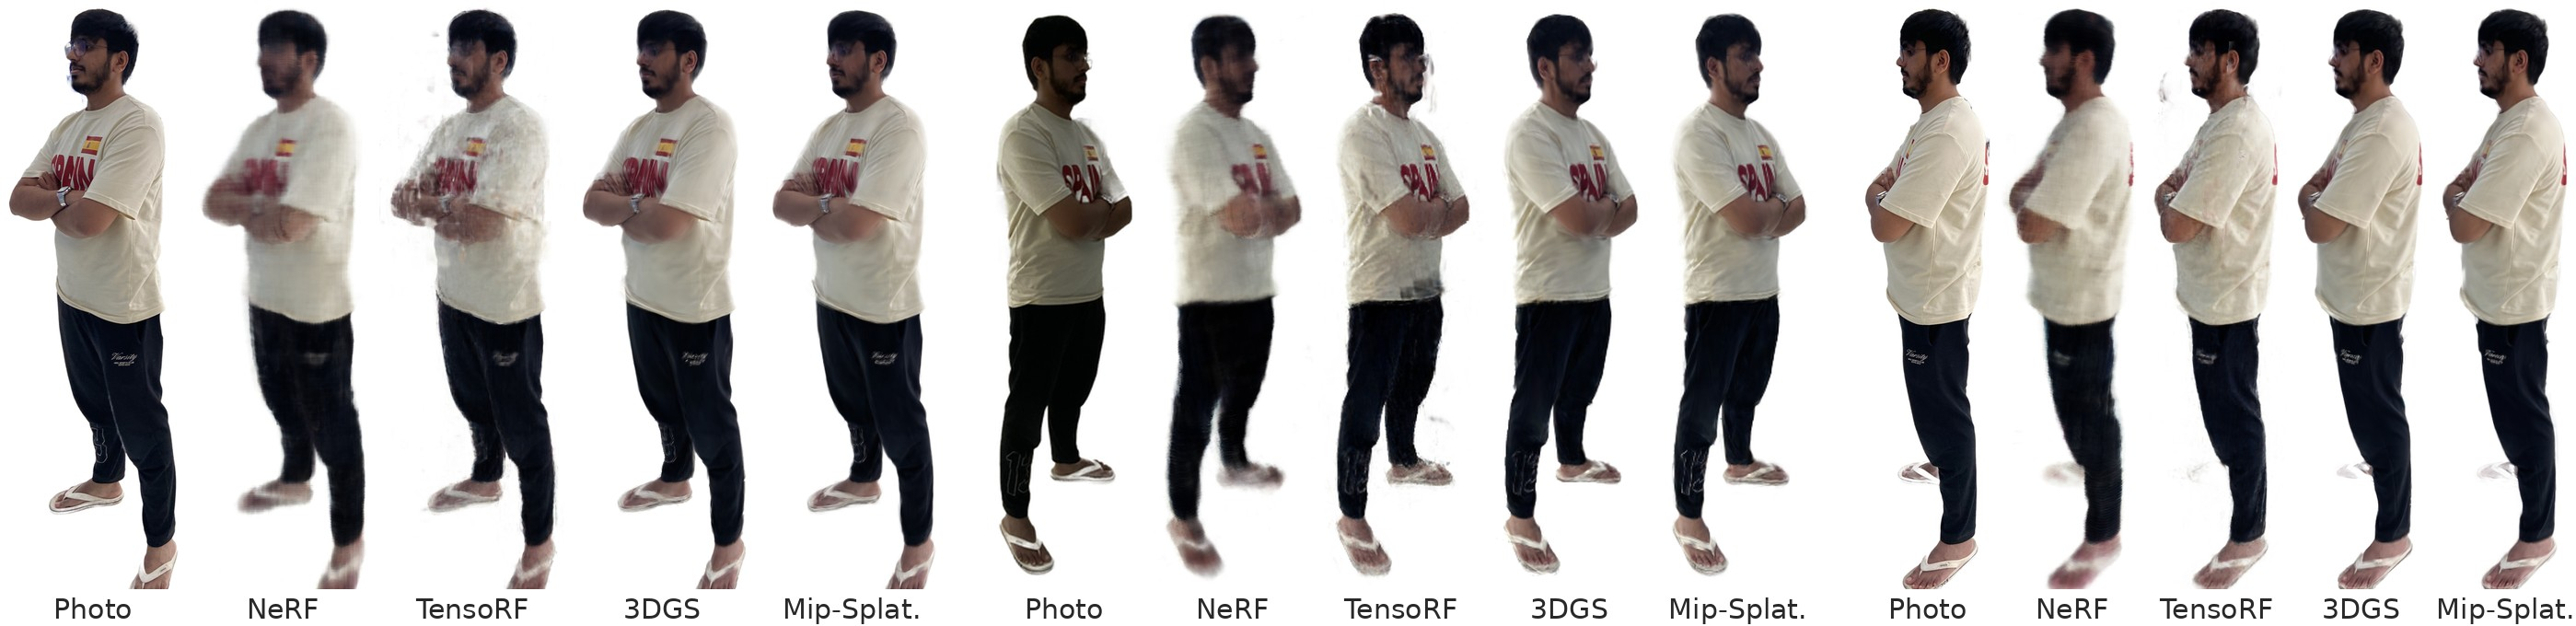
\includegraphics[width=0.86\textwidth]{../figs/fig_strip.jpg}\\[-1pt]
\captionof{figure}{Three of the 16 held-out photos (not used in training) next to each method's render from the same camera.}
\label{fig:teaser}\vspace{3pt}
\begin{minipage}[t]{0.6\textwidth}\centering\resizebox{\linewidth}{!}{\begin{tabular}{@{}lccccccc@{}}\toprule
Method & PSNR$\uparrow$ & SSIM$\uparrow$ & LPIPS$\downarrow$ & Train (min) & FPS$\uparrow$ & Primitives & MB \\\midrule
TensoRF~\cite{chen2022tensorf} & 26.35 & 0.938 & 0.130 & 42 & 1.0 & 17.4M & 67 \\
3DGS~\cite{kerbl20233dgs} & 27.53 & 0.956 & \textbf{0.064} & \textbf{7} & 366 & 195k & 46 \\
Mip-Splatting~\cite{yu2024mip} & \textbf{27.53} & \textbf{0.957} & 0.064 & 10 & \textbf{594} & 217k & 52 \\
\bottomrule\end{tabular}
}
\captionof{table}{Held-out photos (16, $750{\times}1000$): PSNR [dB], SSIM~\cite{wang2004ssim}, LPIPS (VGG)~\cite{zhang2018lpips},
training minutes (runs shared one RTX~5000~Ada), images per second, primitives (Gaussians or network/grid values), MB. Best in bold.}\label{tab:main}
\end{minipage}\hfill
\begin{minipage}[t]{0.37\textwidth}\centering\resizebox{\linewidth}{!}{\begin{tabular}{@{}lcc@{}}\toprule
Rendered at & 3DGS & Mip-Splatting \\\midrule
1/4 size (zoom out) & 24.25 / 0.048 & \textbf{28.63} / 0.028 \\
1$\times$ (training size) & 27.53 / 0.064 & \textbf{27.53} / 0.064 \\
1.6$\times$ (zoom in) & 27.15 / 0.082 & \textbf{27.29} / 0.081 \\
\bottomrule\end{tabular}
}
\captionof{table}{Zoom test: PSNR\,/\,LPIPS rendered at other sizes. Truth: photo averaged down ($\frac14$) or the 1600\,px original ($1.6\times$).}\label{tab:zoom}
\end{minipage}
\end{center}\vspace{-6pt}}]
\thispagestyle{empty}

\section{Task and data}
Draw a person from \emph{new} viewpoints (preset-path video, interactive viewer). Input: only the 125 photos
(four iPhone lenses, video frames) and the cameras Sub-project~1 recovered with VGGSfM~\cite{wang2024vggsfm},
undistorted; person masks give a white background; 1000\,px. Every 8th photo (16) is held out, as in~\cite{kerbl20233dgs}.

\section{Methods}
\paragraph{NeRF~\cite{mildenhall2020nerf} and TensoRF~\cite{chen2022tensorf}}
render a pixel by summing density $\sigma_i$ and colour $c_i$ along its ray, $C=\sum_i T_i(1-e^{-\sigma_i\delta_i})c_i$,
$T_i=\prod_{j<i}e^{-\sigma_j\delta_j}$. NeRF asks one MLP ($8{\times}256$, positional encoding, coarse then fine samples);
TensoRF a 3D feature grid factorised into planes times lines (VM decomposition) and a tiny MLP.
\paragraph{3D Gaussian Splatting~\cite{kerbl20233dgs}}
stores the scene as 3D Gaussians (position, covariance $\Sigma$, opacity, spherical-harmonics colour), started at
100k random points in the scene box and densified while training. Each is projected to a 2D Gaussian
$\Sigma'=JW\Sigma W^\top J^\top$ (EWA splatting~\cite{zwicker2001ewa}), sorted by depth and alpha-blended: real time.
\paragraph{Mip-Splatting~\cite{yu2024mip}}
adds a 3D smoothing filter (no Gaussian finer than the photos sample) and a 2D Mip filter instead of 3DGS's fixed
screen-space dilation, so renders at other zoom levels do not alias.

All use the authors' code (NeRF: nerf-pytorch, the PyTorch port of the original), white background, 30k
iterations; NeRF 1\,h (\NfIters\ steps; the paper 200k+). Extra: 3DGS with the room (\FullPSNR\,dB).

\section{Results}
Table~\ref{tab:main}, Fig.~\ref{fig:teaser}: Mip-Splatting is the most faithful (\MipPSNR\,dB, LPIPS
\MipLPIPS). 3DGS (\GsPSNR) ties NeRF (\NfPSNR) and TensoRF (\TfPSNR\,dB) in PSNR but is far sharper (LPIPS
\GsLPIPS\ vs \NfLPIPS, \TfLPIPS), and the Gaussian methods draw at \GsFPS--\MipFPS\ images per second while the ray
marchers need seconds per image. Table~\ref{tab:zoom} tests the claim of~\cite{yu2024mip}: at a quarter of the size
3DGS falls to \GsZoomOut\,dB, its Gaussians thinner than a pixel, while Mip-Splatting keeps \MipZoomOut\,dB.
Ablation: starting from the Sub-project~1 point cloud instead of random points gives \GsPclPSNR\ (3DGS),
\MipPclPSNR\ (Mip-Splatting) and \FullPclPSNR\,dB (room): it helps 3DGS and the room, not Mip-Splatting.

\section{Interactive viewer in the starter code}
The course's Open3D~\cite{zhou2018open3d} GUI of Sub-project~1 gains a novel-view panel, like
Nerfstudio~\cite{tancik2023nerfstudio}: the 3D view's camera is converted to a pinhole camera, the selected model
is rendered from it on a worker thread and shown behind the scene, so dragging, panning and zooming move the novel
view (preview while moving, full size when still). It shows the held-out photo, exports MP4s along a preset orbit
or keyframes (Catmull-Rom, slerp) and runs our Sub-project~2 Screened Poisson~\cite{kazhdan2013screened} on the open
points, rasterising the mesh in the same view. For laptops without CUDA, the official renderers' inference is
re-done in plain PyTorch (CUDA, Apple MPS, CPU); it matches them at \GsOurs\ and \MipOurs\,dB PSNR (identical).

{\small
\bibliographystyle{ieeetr}
\bibliography{refs}
}
\end{document}
